\chapter{Marco teórico: Autómatas celulares neuronales}

En los últimos años, los autómatas celulares neuronales surgieron como una extensión de los clásicos, con las capacidades de aprendizaje y generalización propias de las redes neuronales artificiales. Esta integración permite que la regla de transición, tradicionalmente fija, sea parametrizable y entrenable mediante técnicas de aprendizaje supervisado.

Las primeras aproximaciones copiaban el funcionamiento de un autómata celular usando una red neuronal convolucional \cite{gilpin2019_nca}. Este método fue dado a conocer por Mordvintsev  et al. \cite{mordvintsev2020_nca}, quienes entrenaron un modelo que aprende de dinámicas locales a partir de ejemplos. Como resultado, las interacciones locales básicas cumplen un objetivo en específico, mostrando propiedades de crecimiento, regeneración, autoorganización y morfogénesis.

Los autómatas celulares neuronales son entonces un tipo de autómatas celulares, pero cuya función de transición está definida como una red neuronal artificial. Retomando las definiciones previas, podemos decir entonces que:

\begin{definition}
	
	Un autómata celular es neuronal si la regla local $\mathcal{R}$ está dada como:
	\[
	\mathcal{R} = F_\theta: \mathbb{R}^{|\mathcal{N}|} \to \mathbb{R}^1
	\]
	donde:
	
	\begin{itemize}
		
		\item $F_\theta$ es una red neuronal parametrizada por $\theta$.
		
		\item $ \theta = \{ w_{uv}, b_v : (u, v) \in E, v \in V \}$ es el conjunto de parámetros entrenables.
		
		\item $\mathbb{R}^{|\mathcal{N}|}$ corresponde al espacio de entrada definido por la vecindad $\mathcal{N}$.
		
		\item $\mathbb{R}^1$ define el valor de salida que representa el nuevo estado de la célula central.
		
	\end{itemize}
	
\end{definition}

La figura \ref{fig:nca} muestra la relación existente entre estas dos tecnologías. En el paso $N$ se tiene una configuración bidimensional con vecindad de Neumann. El estado de cada elemento dentro de la vecindad funciona como valor de entrada para la red neuronal entrenada y devuelve un único resultado. Este resultado corresponde a la salida de la célula central, es decir, a la cual se le está aplicando.

\begin{figure}[!htbp]
	
	\centering
	
	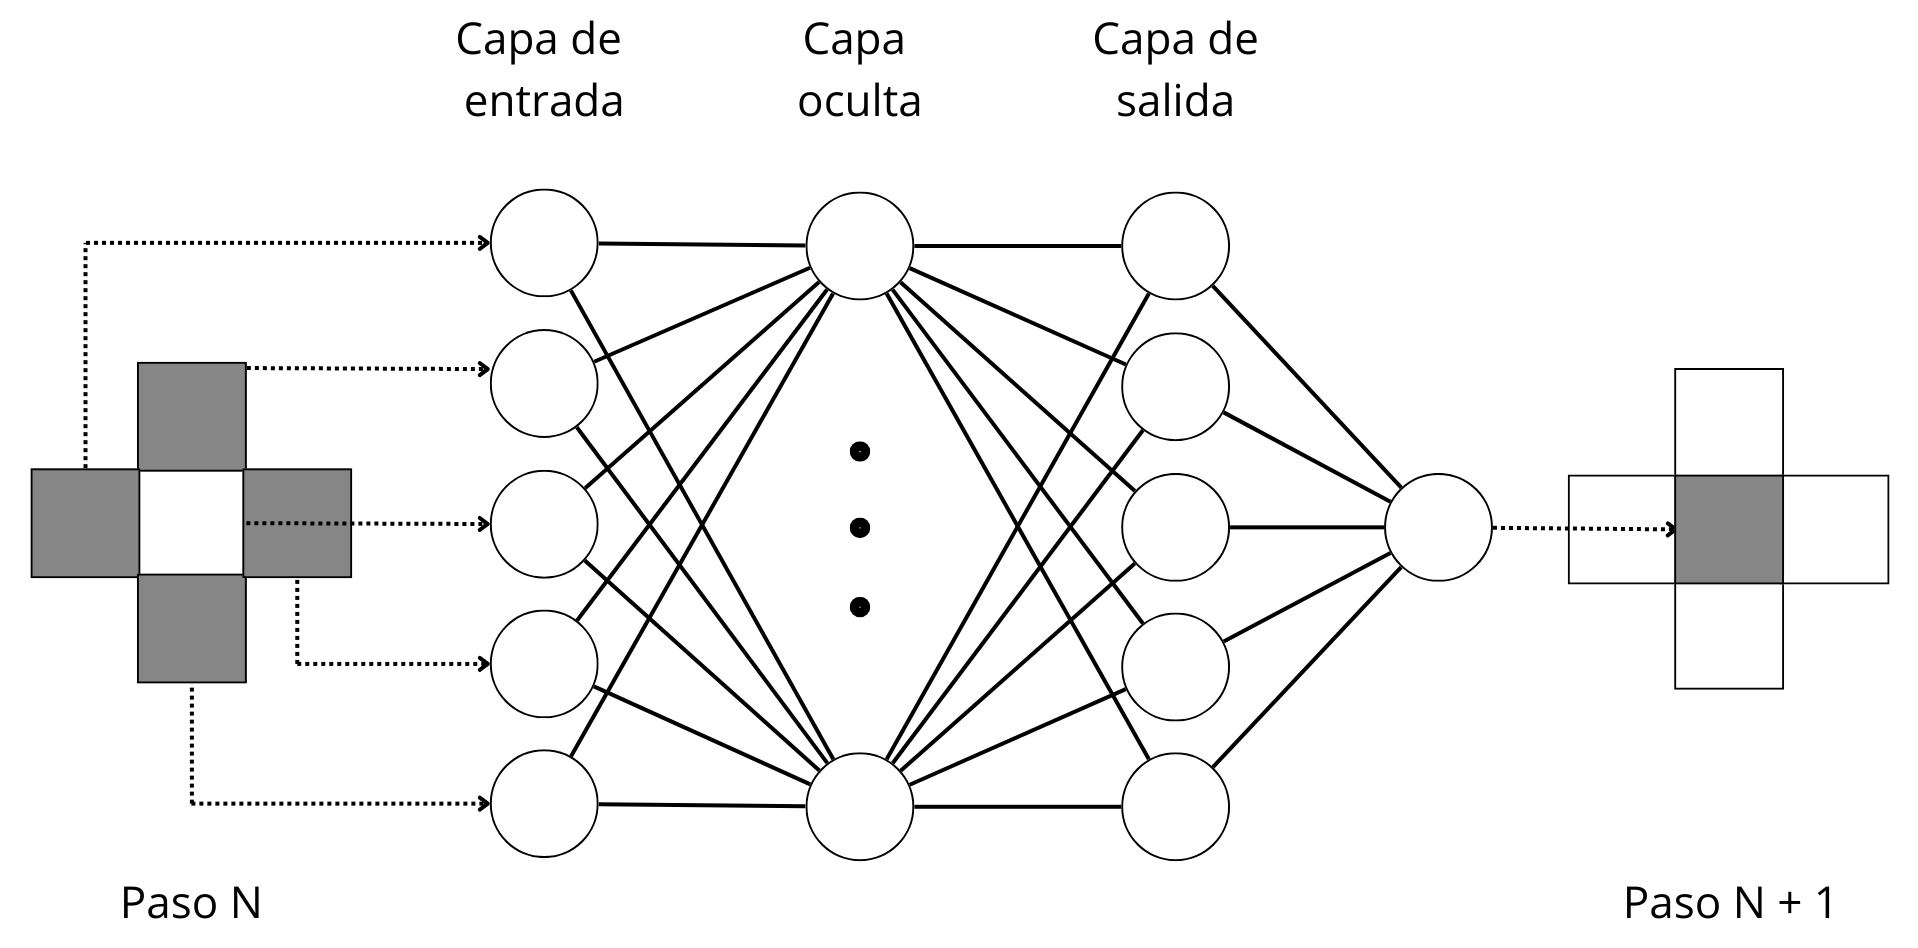
\includegraphics[width=0.8\textwidth]{img/NCA.png}
	
	\caption{Representación gráfica de la red neuronal.}
	
	\label{fig:nca}
	
\end{figure}

Cada célula aplica una misma red neuronal local $F_\theta$ sobre su vecindad inmediata. La entrada de la red consiste en los estados de las celdas dentro de la vecindad y la salida es el nuevo estado de la célula central. 

$F_\theta$ suele representarse como una red neuronal artificial convolucional que permite procesar localmente la información espacial preservando la estructura $D$-dimensional. 

A diferencia de los autómatas clásicos, donde las reglas son explícitas y definidas manualmente, los autómatas celulares neuronales aprenden sus reglas mediante un proceso de entrenamiento. Se establece un grupo de condiciones iniciales $X_0$ y un estado final $X^*$. Luego, la red $F_\theta$ se ajusta para reducir una función de pérdida $\mathcal{L}(X_T, X^*)$, que mide la diferencia entre la configuración obtenida después de $T$ pasos y el estado deseado. Este proceso puede expresarse como:
\[
\theta^* = \arg\min_\theta \mathcal{L}(F_\theta^{(T)}(X_0), X^*).
\]
Durante el entrenamiento, se emplean técnicas de retropropagación a través del tiempo y optimización por gradiente descendente. Esto permite que la red aprenda comportamientos dinámicos complejos, tales como el crecimiento morfológico, la regeneración parcial o la adaptación frente a perturbaciones.

Como las redes neuronales generan valores reales, se puede medir la tasa de error entre la predicción que hacen y el comportamiento real del sistema al usar la regla que han aprendido. Esta métrica de error se propone como base para el desarrollo del presente trabajo. Sin embargo, también se puede comparar la pérdida con otros elementos cercanos, ya que dos células pueden tener muchos vecinos en común, lo que podría explicar el error que se observa en la predicción.

Como se muestra a continuación, esta herramienta ha demostrado ser capaz de generar patrones autoorganizados y adaptativos sin necesidad de una programación explícita de reglas. Algunos ejemplos incluyen:

\begin{itemize}
	
	\item \textbf{Morfogénesis:} Crecimiento de formas y estructuras similares a organismos biológicos.
	
	\item \textbf{Regeneración:} Capacidad de reconstruir regiones dañadas o eliminadas de la configuración.
	
	\item \textbf{Modelado de sistemas complejos:} Simulación de fenómenos físicos, ecológicos o sociales mediante interacciones locales entrenables.
	
\end{itemize}

Esta mezcla de comportamiento que aparece por sí mismo y la habilidad de aprender hace que los autómatas celulares neuronales sean una herramienta muy útil para estudiar sistemas que se organizan solos y que se adaptan.

Los autómatas celulares neuronales surgen de la necesidad de definir funciones de transición más precisas que permitan mejorar la simulación de sistemas complejos, como por ejemplo la propagación del fuego. 

Consideremos un autómata celular bidimensional con tres posibles estados: $\{ materia \; viva, fuego, materia\; quemada \}$, una vecindad de Moore y una función de transición definida por las siguientes reglas: si una célula en estado de materia viva se encuentra adyacente a una célula en estado de fuego, entonces se quema; y si una célula en estado de fuego está rodeada principalmente de materia quemada, entonces se apaga.

Sin embargo, esta formulación que se basa en reglas claras es una simplificación excesiva que reduce la capacidad del modelo para imitar comportamientos que se ven en sistemas reales. Para superar esta limitación, los autómatas celulares neuronales incorporan mecanismos de aprendizaje automático que permiten definir la función de transición de manera adaptativa. 

En este enfoque, el autómata aprende a partir de ejemplos. Por ejemplo, secuencias de video que muestran la propagación del fuego, donde cada estado puede representarse mediante un color y cada célula corresponde a un píxel o conjunto de píxeles. De esta manera, la red neuronal subyacente aprende una función de transición capaz de imitar la dinámica del sistema complejo, ajustando sus parámetros a partir de los datos observados.

Adicionalmente, los autómatas celulares tradicionales suelen operar con configuraciones reducidas, es decir, con pocos estados, vecindades mínimas y reglas básicas, ya que el espacio de configuraciones crece exponencialmente al incrementar cualquiera de estos factores. Esta limitación dificulta modelar sistemas complejos presentes en la naturaleza, los cuales suelen involucrar múltiples variables e interacciones de alta dimensionalidad.

\section{Estado del arte, aplicaciones y líneas actuales de investigación}

Un primer avance en esta línea fue presentado por Gilpin \cite{gilpin2019_nca}, demostrando que una red neuronal convolucional puede aprender el comportamiento de un autómata celular clásico. Su estudio destaca que tanto los autómatas celulares como las redes neuronales convolucionales comparten dos propiedades fundamentales: (1) la actualización basada en una vecindad o \textit{kernel}, y (2) la aplicación simultánea de dicha función en todo el espacio.

En particular, Gilpin entrenó una red neuronal convolucional con un \textit{kernel} de $3 \times 3$ (mismo tamaño que la vecindad de Moore) para imitar el comportamiento del \textit{glider}\footnote{Una de las configuraciones más importantes por su capacidad de moverse en el espacio} en el Juego de la Vida de John Conway. Este trabajo estableció una conexión entre los autómatas celulares y las redes neuronales convolucionales, mostrando que estas redes artificiales pueden actuar como mecanismos de transición local aprendidos.

Posteriormente, esta línea de investigación fue extendida por Mordvintsev et al. \cite{mordvintsev2020_nca}, quienes exploraron representaciones continuas para morfogénesis artificial; y por Niklasson et al. \cite{niklasson2021_nca}, que aplicaron el enfoque a la generación de texturas dinámicas sobre superficies tridimensionales. Otros autores también han sugerido usar autómatas celulares neuronales en robótica, clasificación de patrones y simulación de sistemas fotónicos. Esto ha fortalecido su papel como herramienta para modelar sistemas que se autoorganizan.

\subsection{Morfogénesis}

Mordvintsev diseñó un autómata celular neuronal que permite a una célula crecer para formar un patrón, persistir en el tiempo, regenerarse e incluso rotar. Fue diseñado un modelo que utiliza un autómata celular continuo con un vector de estados de 16 dimensiones. Este modelo incorpora gradientes espaciales utilizando filtros de Sobel. 

\begin{figure}[!htbp]
	\centering
	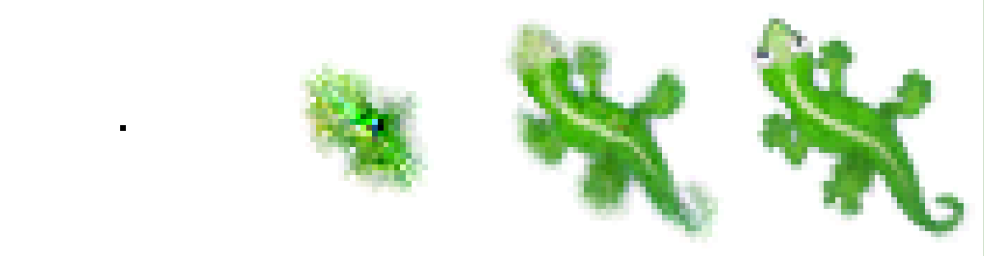
\includegraphics[width=0.6\linewidth]{img/morfogenesis.png}
	\caption{Evolución del \textit{emoji} de una lagartija a partir de una única célula activa después de 219 pasos evolutivos \cite{mordvintsev2020_nca}.}
	\label{fig:morfogénesis}
\end{figure}

El autómata celular neuronal diseñado tiene las siguientes características (las cuales fueron retomadas por múltiples autores que tomaron a \cite{mordvintsev2020_nca} como referencia):

\begin{itemize}
	
	\item El vector de cada célula (cada valor en un rango de $[0,1]$) incluye los canales RGB y un canal $\alpha$ que funciona como umbral para definir si una célula está viva o muerta (establece el resto de valores del vector a $0$ si $\alpha \leq 0.1$). 
	
	Considerando las dimensiones $(\text{largo}, \text{ancho}, 16)$ y un kernel de $3 \times 3$ y se calcula el gradiente en las dos direcciones ($x$ y $y$) usando un filtro Sobel. Esto genera un nuevo vector que se utilizará como entrada para la red neuronal.
	\[ 
	16 (\text{estado propio}) + 16 (\text{gradiente en } x) + 16 (\text{gradiente en } y) = 48 
	\]
	\item Se usaron convoluciones de $1 \times 1$ con una función \textit{ReLU} y alrededor de $8000$ parámetros entrenables y devuelve un $\delta$ que se suma al estado actual de célula antes del siguiente paso. 
	
	
	
	\item Se omite el cálculo para las células muertas y la actualización de cada célula se realiza con una probabilidad del $50\%$. La actualización debe ser estocástica para lograr un mejor rendimiento \cite{niklasson2021_nca}. 
	
\end{itemize}

Eyvind Niklasson et al. \cite{niklasson2021_nca} compararon el rendimiento del modelo en \cite{mordvintsev2020_nca} con actualización síncrona y asíncrona. Donde, tras haber llevado a cabo pruebas con diferentes tamaños de paso, concluyeron que la función de pérdida crece exponencialmente cuando la actualización es síncrona. Sin embargo, esto ocurre únicamente cuando el tamaño de paso es mayor que uno.

Una hipótesis de este comportamiento es que, al tener células que se actualizan en diferentes periodos de tiempo, cada célula puede conocer parte del contexto de su vecindad. Esto no se logra únicamente conociendo los valores actuales de cada vecino.

Se realizaron los siguientes experimentos en \cite{mordvintsev2020_nca}:

\begin{enumerate}
	
	\item Crecer una única célula activa para formar una figura dada mediante \textit{backpropagation}. Cuando el autómata celular llega a la figura deseada, si se siguen aplicando las reglas de evolución, puede crecer sin límites, quedarse en la misma figura, eliminar todas las células o crear patrones que son caóticos o que se repiten.
	
	
	
	\item Convertir las figuras objetivo en atractores usando \textit{sample pool}. Se entrenó mediante múltiples condiciones iniciales, obtenidas a partir de entrenamientos fallidos, para llegar al objetivo desde diferentes configuraciones. 
	
	
	
	\item Regenerar partes de la figura. Se eliminaron partes de la figura objetivo y se añadieron al conjunto de entrenamiento.
	
	
	
	\item Rotaron la figura objetivo. Dado que los filtros de Sobel funcionan como direcciones ortogonales, se puede aplicar una rotación mediante: 
	\[ \begin{bmatrix}
		K_x & K_y
	\end{bmatrix} = \begin{bmatrix}
		cos \theta & -sin \theta \\
		sin \theta & cos \theta
	\end{bmatrix} \cdot \begin{bmatrix}
		Sobel_x & Sobel_y
	\end{bmatrix} \]
	Para modificar el ángulo sin necesidad de reentrenar el modelo.
	
\end{enumerate}

\subsubsection{Autómatas celulares neuronales isotrópicos}

En \cite{mordvintsev2022_iso_nca}, \cite{mordvintsev2022_iso_nca2} y \cite{mordvintsev2023_snca}, Mordvintsev et al. presentan una nueva configuración que no tenga una dirección preferida, la cual nombraron autómatas celulares neuronales isotrópicos.

Para que esta regla sea isotrópica, es necesario que sea independiente de la dirección (sin distinguir ``arriba'' de ``izquierda''). Esto permite crear rotaciones o simetrías sin que el sistema se descontrole.

Se sustituyen las funciones de los filtros de Sobel en \cite{mordvintsev2020_nca} por un único filtro laplaciano:
\[
K_{lap} = \begin{bmatrix}
	1 & 2 & 1 \\
	2 & -12 & 2 \\
	1 & 2 & 1 	
\end{bmatrix}
\]
El cual se concatena al vector de cada célula y alimenta a una red neuronal artificial de $9408$ parámetros. 

A continuación, se describen los resultados obtenidos con dos diferentes enfoques:
\begin{enumerate}
	\item Estrategia de semilla estructurada: Se necesitan al menos tres células con valores diferentes y no colineales para definir la orientación y la posición. Modificar la posición de estos puntos implica una evolución acorde a la posición de los mismos.
	
	\item Estrategia de una única semilla: Se modifica la función de pérdida para que sea invariante ante rotaciones y reflejos. Para evitar comparar la figura resultante con todas las rotaciones posibles, se mapean ambas figuras a coordenadas polares y, para cada posible ángulo de rotación, se calcula la diferencia. Para disminuir la complejidad computacional, se aplica la transformada rápida de Fourier y se hace uso del teorema de la convolución:
	\[
	s * t = \mathcal{F}^{-1} (\mathcal{F}(S) \cdot \mathcal{F}(T)) 
	\]
	Se obtienen todas las diferencias únicamente como una multiplicación de transformadas.
	
	Para evitar que se formen patrones simétricos mezclados (como figuras con cabeza-cabeza o cola-cola), se agrega un nuevo canal llamado \textit{binary auxiliary channel} que da valores de $-0.5$ y $0.5$ a la parte superior e inferior de la imagen, respectivamente.
	
	Con estas nuevas configuraciones se puede obtener el mismo resultado que en \cite{mordvintsev2020_nca}, pero sin la dependencia de una dirección explícita y con una red neuronal artificial con menos parámetros.
	
\end{enumerate}

\subsubsection{Autoclasificación}

En \cite{mordvintsev2020_mnist} Mordvintsev utiliza los autómatas celulares neuronales para la autoclasificación de MNIST\footnote{Conjunto de datos de imágenes $28 \times 28$ de números en el rango $[0,9]$} las cuales fueron binarizadas con un umbral de $0.1$. 

El objetivo es que, a partir de una configuración inicial de células vivas, el sistema pueda reconocer la forma solo usando reglas locales. En este caso, se trata de identificar los números de MNIST.

Estos son los cambios del autómata celular MNIST respecto al modelo original \cite{mordvintsev2020_nca}:

\begin{itemize}
	
	\item Vector de la célula: Originalmente se usaban los canales RGB; ahora se emplean 10 canales que funcionan como distribución de probabilidad de cada posible número. Durante la evaluación se utiliza el mayor de ellos.
	
	\item Célula viva o muerta: En \cite{mordvintsev2020_nca} se define mediante el canal $\alpha$, pero las células muertas siguen siendo visibles para el resto. En \cite{mordvintsev2020_mnist}  únicamente interactúan las células vivas.
	
	\item Topología: Todas las células son un único componente conexo.
\end{itemize}

Con el nuevo modelo, Mordvintsev pudo realizar clasificaciones con una precisión del $95.3\%$ con una función de pérdida $L_2$ y ruido añadido. Este experimento demostró que los autómatas celulares neuronales no solo pueden generar patrones y autorregenerarse, sino también realizar tareas de clasificación distribuidas sin una capa de decisión global.

Aunque los modelos en \cite{mordvintsev2020_nca} y \cite{mordvintsev2020_mnist} son robustos frente a diferentes tipos de perturbaciones, su comportamiento se puede ver afectado por estados individuales de las células, parámetros del modelo y el campo perceptivo (la manera en cómo las células perciben su vecindad).

Es por esto que Randazzo et al. \cite{mordvintsev2021_a_nca} buscan enfrentar estrategias adversarias en el mismo espacio celular para estudiar la reprogramación de los autómatas celulares mediante dos experimentos:
\begin{enumerate}
	\item \textbf{Inyección de adversarios}: Se entrena un nuevo modelo de autómata celular, que se coloca en el entorno que ejecuta uno de los modelos originales, para secuestrar el comportamiento del colectivo.
	
	\item \textbf{Perturbación de estados}: A un modelo ya entrenado, se le aplican perturbaciones a todas las células del sistema de forma simultánea.
\end{enumerate}

Para la inyección de adversarios se utilizan dos modelos: el modelo original del autómata celular para MNIST con probabilidad de $90\%$ y un nuevo modelo que clasifica a todos los números como ``ocho'' ($10\%$).  Se introducen varias células invasoras en figuras que ya han sido clasificadas, y estas células muestran un comportamiento dominante al clasificar todos los elementos como ``ocho''. Además, una vez retiradas las células invasoras, el sistema es capaz de recuperarse la mayoría de las veces.

Sin embargo, al aplicar el mismo procedimiento para \cite{mordvintsev2020_nca}, los resultados no tuvieron el mismo rendimiento. Probaron modificar la morfología de la imagen de una lagartija sin cola y con otro color, pero ninguna estrategia fue capaz de invadir por completo el modelo original. 

Una hipótesis es que para MNIST no necesita cambiar completamente su valor para producir algo diferente de lo que generaba antes, ya que el estado de la mutación es un estado que el modelo original ya tenía en cuenta. Por otro lado, al cambiar el color y la forma en \cite{mordvintsev2020_nca}, se están explorando configuraciones nunca antes vistas por el modelo original.

Para el segundo experimento (perturbación de estados), se sigue la línea de modificar el color y la forma de la imagen de una lagartija. Se aplica una perturbación global de estados cada paso de tiempo con el objetivo de identificar la perturbación específica que dé como resultado un patrón estable.

En cada paso evolutivo, se multiplica el vector de cada célula por una matriz simétrica $A$ de $16 \times 16$ \cite{mordvintsev2020_nca}. Para definir los valores de la matriz, se inicia con una matriz simétrica $I$ y, a diferencia del modelo original, la configuración inicial se establece como la figura objetivo del mismo.

Esta configuración permite crecer un sistema con perturbaciones, alterar su forma y color una vez crecido y modificar el impacto y el número de perturbaciones posibles. Al manejar matrices simétricas, se puede representar como 
\[A = Q \Lambda Q^T\] 
donde: 

\begin{itemize}
	
	\item $\Lambda$ es la matriz diagonal de los valores propios.
	
	\item $Q$ es la matriz unitaria de los vectores propios.
	
\end{itemize} 

Si $\Lambda = I \to A = I$, por lo que no existe perturbación (multiplicación por matriz identidad). Bajo esta premisa, se propone la siguiente fórmula:
\[ A_k = Q(kD + I)Q^T\]
Donde:

\begin{itemize}
	
	\item $A$ es la matriz original.
	
	\item $k$ es el factor de escala.
	
	\item $D$ es la dirección de la perturbación $\Lambda - I$ en el espacio de valores propios. 
	
\end{itemize}

Si $k = 0$, no existe perturbación en el sistema:

\begin{gather*}
	A_k = Q(0D + I)Q^T \\
	A_k = Q I Q^T
\end{gather*}

Si $k = 1$, se conserva la perturbación original:

\begin{gather*}
	A_k = Q(1D + I)Q^T \\
	A_k = Q(\Lambda - I + I)Q^T \\
	A_k = Q \Lambda Q^T
\end{gather*}

Mostrando que se puede escalar el tamaño de la perturbación, incluso con perturbaciones inversas con $k = -1$.

Si consideramos dos perturbaciones cuyos vectores propios son similares: $A_k = Q(k_AD_A + I)Q^T$ y $B_k = Q(k_B D_B + I)Q^T$, podemos combinarlos como
\[ comb(A_k, B_k) = Q (k_A D_A + k_B D_B + I) Q^T = k_A A + k_B B + (1 - k_A - k_B) I \]
Esta nueva combinación permite configurar múltiples perturbaciones, las cuales se vuelven más sensibles conforme aumentan los $k$.

Estos experimentos muestran cómo los autómatas celulares neuronales pueden ser vulnerables a diferentes estrategias y cómo las mutaciones ``exactas'' pueden modificar la estructura de todo el sistema.

Todas estas representaciones han tenido lugar en un espacio bidimensional. A continuación se presentan algunas propuestas en espacios tridimensionales. 

\subsubsection{Representaciones tridimensionales}

Zhang et al. \cite{zhang2021_gca} proponen un modelo generativo tridimensional denominado autómata celular generativo que extiende el paradigma de los autómatas celulares hacia la generación progresiva de formas tridimensionales. A diferencia de enfoques que intentan reconstruir directamente la forma completa, el autómata celular generativo formula el proceso como una cadena de Markov, donde cada paso corresponde a una transición local sobre una rejilla tridimensional. 

El modelo se entrena para que estas reglas locales, al repetirse, converjan hacia formas específicas. Para ello, se representa la forma como puntos de superficie en una rejilla 3D y se emplea una red convolucional dispersa que opera únicamente sobre las regiones activas.

Durante el entrenamiento, se utilizan secuencias ligeramente distintas a las cadenas de muestreo reales, pero que convergen hacia las formas del conjunto de datos. Esto permite que el modelo aprenda reglas de transición robustas, capaces de generar formas diversas desde configuraciones parciales. Con una sola inferencia, el sistema puede tomar diferentes ejemplos de la distribución que ha aprendido, obteniendo buenos resultados en tareas de completar y generar formas en 3D.

Este enfoque es una aportación importante a la morfogénesis computacional, ya que muestra que las reglas locales que se autoorganizan pueden aplicarse a estructuras 3D complejas utilizando redes neuronales adaptadas.

En \cite{zhang2021_gca}, se muestra que la autoorganización local se puede escalar a tres dimensiones. Por otro lado, Shyam Sudhakaran et al. \cite{sudhakaran2021_nca_3d} amplían el trabajo de \cite{mordvintsev2020_nca} a tres dimensiones, usando el juego de Minecraft como espacio celular\footnote{En Minecraft, se pueden crear estructuras estáticas (como árboles) y dinámicas (como máquinas voladoras)}. El autómata celular neuronal entrenado puede crear estructuras de hasta 3584 bloques utilizando 50 bloques diferentes, manteniendo las propiedades de regeneración de su versión en 2D.

Una entidad en Minecraft se representa como una red 3D donde cada elemento es un vector que almacena (1) el tipo de bloque (incrustado en un vector \textit{one-hot}), (2) su estatus (replicando el comportamiento del canal $\alpha$ de \cite{mordvintsev2020_nca}) y (3) estados ocultos.

Se utilizan convoluciones para permitir la generación y manipulación de estructuras 3D. Además, se sustituye el uso de filtros de Sobel por una red de percepción aprendible con un kernel de $3 \times 3 \times 3$, \textit{stride}\footnote{Cuántas posiciones se desplaza el \textit{kernel} sobre la entrada en cada operación de convolución} de 1 y canales de salida equivalentes a tres veces el número de canales del estado celular. Esta red permite que el sistema aprenda activamente a percibir su entorno local, adaptando sus filtros durante el entrenamiento y capturando patrones espaciales relevantes de manera dinámica.

Se utiliza una actualización estocástica y un umbral de activación similar a \cite{mordvintsev2020_nca}. Finalmente, todos los modelos se inicializan con una distribución normal estándar, con media cero y desviación estándar en el rango de $0.0001$ a $0.1$, lo que proporciona un punto de partida estable para el entrenamiento y la evolución del sistema. Este sistema hereda las propiedades regenerativas de su versión 2D.

Finalmente, Horibe et al. \cite{horibe2021_softrobot} llevan las propiedades regenerativas al mundo físico. Se implementa el enfoque regenerativo en robots blandos mediante autómatas celulares neuronales. Cada robot tiene un conjunto de volúmenes de reposo para cada vóxel\footnote{Unidad básica de un espacio tridimensional, similar a un píxel en imágenes 2D, pero con volumen}. Estos volúmenes se activan con una señal global que tiene forma de onda sinusoidal, lo que causa que se expandan y se contraigan. Esta dinámica permite simular locomoción a través de ciclos de actuación, evaluando el desplazamiento del centro de masa como métrica de fitness. Los robots blandos se componen de distintos tipos de vóxeles: músculos en fase y contrafase, huesos rígidos y flexibles, cada uno con un rol en la locomoción.

El modelo entrenado demuestra que los robots blandos pueden recuperar parcialmente su morfología original tras sufrir daño y restaurar su capacidad de movimiento sin intervención externa. Este comportamiento surge de la dinámica autoorganizada del autómata celular neuronal, que codifica de manera implícita la forma objetivo y su capacidad de reparación.

Para evaluar la capacidad de locomoción y regeneración de los robots blandos generados mediante autómatas celulares neuronales, se emplea el simulador físico Voxelyze. Los experimentos se realizan en configuraciones 2D y 3D, utilizando rejillas de $7 \times 7$ y $9 \times 9 \times 9$ vóxeles, respectivamente. Las condiciones de frontera tipo Dirichlet limitan el crecimiento morfológico a regiones internas ($5 \times 5$ en 2D y $7 \times 7 \times 7$ en 3D).

Este entorno permite comprobar cómo los autómatas celulares neuronales se autoorganizan para crear formas que son funcionales y resistentes. Además, proporciona una base cuantitativa para comparar la eficiencia locomotora antes y después de procesos de regeneración. La estructura en vóxeles ayuda a combinar reglas locales y programación distribuida, y se relaciona con modelos inspirados en la biología sobre cómo se forma la estructura.

En conjunto, estos trabajos evidencian cómo los autómatas celulares neuronales pueden extender sus principios regenerativos y de autoorganización a dominios tridimensionales cada vez más complejos. Mientras Autómatas celulares generativos establecen un marco generativo para formas 3D a partir de reglas locales aprendidas, los experimentos en Minecraft muestran que dichas propiedades pueden preservarse incluso en entornos con alta variabilidad estructural. Finalmente, la aplicación en robots blandos confirma el potencial bioinspirado de los autómatas celulares neuronales: no solo permiten generar morfologías funcionales, sino que además dotan a los sistemas físicos de resiliencia ante daños, abriendo camino hacia formas de robótica autorreparable.

Otra forma de implementar los autómatas celulares neuronales en 3D es mediante planos, mallas y texturas autoorganizadas que cubren la superficie de un objeto tridimensional. 

\subsection{Autómata celular neuronal en malla}

Niklasson et al. \cite{mordvintsev2021_mnca} y Mordvintsev et al. \cite{mordvintsev2021_mnca2} \cite{mordvintsev2021_unca} introducen el concepto de texturas autoorganizadas, cuyo objetivo es reproducir la apariencia global de una textura de referencia sin generar copias exactas. Para esto, entrenan un autómata celular neuronal utilizando la misma estructura neuronal que se propuso en \cite{mordvintsev2020_nca}, para que pueda reconocer y crear patrones distintivos como tableros de ajedrez, líneas o mosaicos. Aunque este enfoque tiene un carácter demostrativo, constituye una evidencia significativa de que los autómatas celulares neuronales pueden aprender y generalizar comportamientos visuales locales en lugar de memorizar imágenes específicas.

Niklasson et al. proponen los autómatas celulares neuronales en mallas \cite{mordvintsev2024_mesh_nca}, que es un método creado para crear texturas en movimiento en superficies en 3D. A diferencia de los experimentos en cuadrículas de dos dimensiones, los autómatas celulares neuronales en mallas aplican el mecanismo de autoorganización a mallas de cualquier forma, incluso si están en movimiento. El modelo es consistente en diferentes situaciones, es resistente a cambios externos y permite ajustar características como la densidad, la dirección y la rotación de los patrones que aparecen. Además, varios autómatas celulares neuronales en redes pueden combinarse, creando cambios suaves entre texturas sin interrupciones.

\begin{figure}[!htbp]
	
	\centering
	
	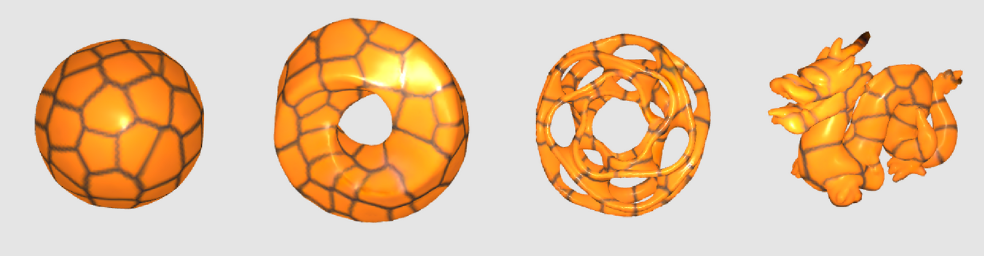
\includegraphics[width=0.75\linewidth]{img/mesh.png}
	
	\caption{El entrenamiento se realiza sobre un poliedro simétrico y el autómata celular neuronal puede ser extrapolado a cualquier objeto tridimensional \cite{mordvintsev2020_nca}.}
	
	\label{fig:mesh}
	
\end{figure}

Sin embargo, este enfoque presenta un reto de escalabilidad. El número de células involucradas suele encontrarse en el rango de $10^4 \sim 10^5$, lo que limita la resolución alcanzable a entre $64 \times 64$ y $256 \times 256$ píxeles. Como el tiempo de entrenamiento escala de forma cuadrática con respecto al número de celdas, el aumento de resolución conlleva un cuello de botella en la propagación de información a lo largo de la malla.

Para solucionar esta limitación, Niklasson et al. sugieren en \cite{mordvintsev2024_mesh_nca2} un modelo híbrido que une autómatas celulares neuronales  con representaciones neuronales implícitas. La idea central es desacoplar el tamaño de la cuadrícula de los autómatas celulares neuronales  de la resolución final, delegando el renderizado detallado a un decodificador ligero denominado red local de producción de patrones. De este modo, el autómata celular neuronal mantiene una cuadrícula explícita y relativamente pequeña que evoluciona de manera local, mientras que la red local de producción de patrones se encarga de producir el color en cualquier punto del espacio continuo a partir de información interpolada de las celdas vecinas.

En términos formales, para cada punto de muestreo $p$, la red local de producción de patrones recibe dos entradas: Una es un estado celular promedio $s(p)$, obtenido mediante interpolación de las celdas cercanas en un primitivo geométrico; la otra es un vector de coordenadas locales $u(p)$, que codifica la posición relativa de $p$ dentro de dicho primitivo. Dependiendo de cómo se divida el espacio, estas formas básicas pueden ser rectángulos, cubos, triángulos o polígonos en general. Estas formas están definidas por coordenadas $\lambda_i(p)$ que deben cumplir con ciertas propiedades, como ser una partición unitaria y no ser negativas. Para asegurar una continuidad en el espacio, se cambian las coordenadas usando funciones sinusoidales en cuadrículas cartesianas o en redes triangulares, creando así campos posicionales suaves.

El resultado es un sistema que conserva las propiedades autoorganizativas de los autómatas celulares neuronales al tiempo que permite alcanzar mayor resolución sin un aumento proporcional del costo computacional. Desde una perspectiva biológica, el autómata celular neuronal puede interpretarse como un plano morfogenético que define la organización global, mientras que la red local de producción de patrones añade los detalles finos sin necesidad de simular interacciones locales a gran escala. Este paralelismo, aunque principalmente ilustrativo, refuerza la idea de que los autómatas celulares neuronales pueden actuar como generadores de estructuras robustas y adaptables, mientras que módulos complementarios aportan precisión y escalabilidad.

A pesar de estas mejoras, una limitación persistente es que cada autómata celular neuronal debe entrenarse de manera específica para una textura o patrón dado. Incluso en escenarios donde múltiples autómatas celulares neuronales coexisten, cada modelo requiere su propio entrenamiento independiente. Esto ha motivado nuevas propuestas orientadas a la construcción de espacios compartidos de autómatas celulares neuronales, capaces de generalizar a múltiples texturas dentro de un mismo marco de entrenamiento.

\subsection{Modelos generativos}

Cada imagen creada con un autómata celular neuronal tiene una red neuronal artificial que ha sido entrenada específicamente para copiar ese comportamiento. Alejandro Hernández et al. \cite{hernandez2021_ncam} proponen unas redes neuronales artificiales de mayor capacidad que permitan crecer múltiples imágenes, a lo que llamaron colector de autómatas celulares neuronales.

El colector de autómatas celulares neuronales usa un modelo de convoluciones dinámicas para modelar un espacio de dichos autómatas. Utiliza un \textit{autoencoder} que se compone de un codificador y un decodificador: El codificador transforma la entrada en una representación continua y luego categórica, que el decodificador reconstruye en el espacio original.

Un elemento destacable de la arquitectura propuesta es un parámetro entrenable llamado \textit{Leak Factor} (LF) que mejora la estabilidad durante el entrenamiento. Este parámetro regula la cantidad de información que se filtra en cada paso del modelo; por ejemplo, un valor bajo retiene el conocimiento acumulado. Este valor se incrementa durante el entrenamiento a medida que mejora el rendimiento.

La arquitectura también emplea convoluciones dinámicas. Los \textit{kernels} se generan a partir del \textit{embedding} de cada instancia, permitiendo adaptabilidad sin modificar la estructura del autómata celular neuronal. El colector de autómatas celulares neuronales inicia desde una imagen semilla y actualiza cada celda mediante percepciones locales (filtros Sobel $+$ normalización) y capas densas por píxel, moduladas por el LF. Se exploran actualizaciones estocásticas y sincrónicas, siendo esta última más precisa y estable, tal como en \cite{niklasson2021_nca}.

Los experimentos muestran que la codificación y la actualización simultáneamente mejoran la calidad de la reconstrucción, incluso sin mecanismos de enmascaramiento. También se observa que aumentar la dimensionalidad del \textit{embedding} mejora significativamente los resultados.

Por otro lado, Kevin Frans en \cite{frans2021_stampca} propone un modelo llamado autómatas celulares neuronales condicionales, cuya semilla recibe un \textit{embedding}, el cual define la imagen en la cual va a crecer. 

Dado un diseño deseado, una red de codificador lo comprime en un \textit{embedding}, el cual se utiliza como condición inicial en el autómata celular neuronal, que luego itera para crecer en la figura objetivo; esto permite crear nuevas configuraciones.

Utilizando un \textit{dataset} con aproximadamente 3000 \textit{emojis} de $32 \times 32$ píxeles, fue capaz de entrenar a un autómata celular neuronal condicional utilizando el mismo método de \cite{mordvintsev2020_nca} para poder dibujar todos los \textit{emojis} con un único autómata celular neuronal.

Para generar números de MNIST, se adopta un enfoque tipo red adversarial generativa, donde el objetivo es crecer dígitos desde ruido aleatorio. Dado que entrenar directamente un autómata celular neuronal como generador de red adversarial generativa resultó inestable, se utilizó una estrategia en dos etapas: (1) Se entrena primero un generador tradicional (\textit{feedforward}) para mapear vectores aleatorios a dígitos MNIST y (2) el autómata celular neuronal se entrena para imitar la salida de ese generador, logrando una generación más estable.

Este enfoque permite que el autómata celular neuronal genere dígitos sin necesidad de un \textit{dataset} explícito, aprendiendo directamente a partir del objetivo de la red adversarial generativa. Además, se observa un patrón de crecimiento distintivo: mientras los \textit{emojis} crecen en ondas desde el centro, los dígitos MNIST se desarrollan siguiendo la forma del trazo.

Mingxiang Chen et al. \cite{chen2020_vaenca} combinan los principios de codificador automático variacional con autómata celular neuronal. Utilizan un \textit{encoder} que transforma una imagen en una distribución de probabilidad, las cuales forman un \textit{embedding}, el cual funciona como condición inicial del autómata celular neuronal. Después, Rasmus Berg Palm et al. \cite{rasmus2022_vnca} llaman a este modelo ``autómatas celulares neuronales variacionales''. También afirman que ninguno de los otros modelos mencionados (\cite{mordvintsev2020_nca}, \cite{hernandez2021_ncam}, \cite{zhang2021_gca}, \cite{horibe2021_softrobot} y \cite{frans2021_stampca}) es realmente generativo.

El autómata celular neuronal variacional aprende una distribución de probabilidad que codifica los datos observados. A partir de esta representación, el \textit{encoder} genera imágenes mediante un autómata celular neuronal que simula el crecimiento espacial desde una semilla. A diferencia del codificador automático variacional, que decodifica la imagen directamente, el autómata celular neuronal variacional utiliza el \textit{embedding} como configuración inicial de una cuadrícula de celdas que evolucionan siguiendo las reglas definidas por una red neuronal convolucional. 

Por otra parte, este modelo incorpora mecanismos de duplicación celular inspirados en la mitosis. Cada $M$ pasos, las celdas se duplican hacia la derecha y hacia abajo, permitiendo a la imagen crecer de manera autoorganizada. 

Los experimentos realizados en \cite{rasmus2022_vnca} demuestran que el autómata celular neuronal variacional es capaz de aprender procesos generativos autoorganizados tanto en dominios simples como MNIST, como en conjuntos más complejos como CelebA\footnote{\textit{Dataset} de imágenes de celebridades}. En MNIST, el modelo logra reconstrucciones precisas y muestras plausibles desde el espacio latente, con una log-verosimilitud de $\log p(x) \geq -84.23$ nats\footnote{Unidad de medida utilizada en aprendizaje automático y estadística para expresar la $\log$-verosimilitud o la entropía de un modelo}; su rendimiento es comparable a modelos autorregresivos como PixelCNN. Además, el análisis del espacio latente muestra una estructura más clara y organizada en comparación con los decodificadores convolucionales tradicionales. Esto indica que la codificación es más semántica y eficiente.

En CelebA, aunque las muestras generadas directamente no alcanzan calidad visual comparable a modelos de última generación, el autómata celular neuronal variacional muestra capacidad de reconstrucción robusta y mejora visual significativa al ajustar el parámetro $\beta$, que regula el equilibrio entre fidelidad de reconstrucción y calidad de generación. 

Finalmente, se explora la resiliencia de los autómatas celulares neuronales variacionales ante daño estructural durante el crecimiento. Al eliminar las capas de duplicación y entrenar con un esquema de recuperación de daño, el modelo aprende dinámicas estables capaces de restaurar imágenes deterioradas casi por completo, incluso tras múltiples pasos de evolución. Este comportamiento sugiere que el autómata celular neuronal variacional no solo codifica la imagen, sino que también es un proceso de reconstrucción en el estado celular.

\subsection{Representaciones y aplicaciones adicionales}

Hasta ahora, muchos de los estudios sobre autómatas celulares neuronales se han enfocado en la morfogénesis, que es el proceso de formación de formas, y en su habilidad para crear estructuras visuales que se organizan solas. Sin embargo, también han surgido enfoques que amplían el marco conceptual hacia nuevas formas de representación y aplicaciones en dominios específicos. A continuación, se presentan algunas de estas variantes.

Mattie Tesfaldet et al. \cite{Tesfaldet2022_vitca} extienden los autómatas celulares neuronales mediante mecanismos de atención inspirados en arquitecturas de \textit{transformers}, dando lugar a autómatas celulares con \textit{transformers} de visión. Esta arquitectura híbrida permite que las interacciones locales tengan acceso contextual a regiones más amplias a través de \textit{self-attention}, lo que habilita organización global sin incurrir en la complejidad cuadrática típica de la atención completa. Los autómatas celulares con \textit{transformers} de visión adaptan el proceso de los \textit{transformers} de visión tradicionales, que dividen una imagen en parches y los convierten en secuencias de \textit{tokens}, al formato de una cuadrícula de celdas, donde cada celda almacena información visual, posicional y oculta. En lugar de aplicar atención global, restringe el cálculo a vecindarios locales, manteniendo así la naturaleza distribuida del sistema y reduciendo el costo computacional. El entrenamiento se realiza de forma iterativa, alternando entre inyectar entradas corruptas y actualizar parcialmente los estados celulares hasta reconstruir la imagen. De este modo, los autómatas celulares con \textit{transformers} de visión combinan eficiencia, capacidad de autoorganización y organización espacial coherente.

En un ámbito distinto, Jian Tang et al. \cite{Jian2023_nca} emplean una red neuronal convolucional para simular el desarrollo de microestructuras en la solidificación de metales. Cada celda del dominio contiene un estado de fase $P\in[0,1]$ (donde $p=0$ representa líquido y $p=1$ sólido), tres ángulos de Euler $\theta=(\alpha_1,\alpha_2,\alpha_3)$ que definen su orientación cristalográfica y la magnitud de subenfriamiento $\Delta T=T_{melting}-T$. La evolución se modela con un autómata celular neuronal que aplica recurrentemente una red neuronal convolucional para predecir los incrementos en fase, orientación y estados ocultos. Estos canales ocultos facilitan el aprendizaje de patrones temporales complejos sin necesidad de reglas explícitas. Con ello, el modelo reproduce fenómenos como crecimiento competitivo o direcciones preferentes, con una eficiencia computacional sustancialmente mayor que la de muchos autómatas celulares tradicionales y con capacidad de generalización fuera del rango de entrenamiento.

Por otro lado, Gordon H. Y. Li et al. \cite{li2024_pnca} proponen el modelo de autómatas celulares neuronales fotónicos, que aprovecha la velocidad y la interconexión masiva de la fotónica para implementar autómata celular neuronal en hardware óptico. A diferencia de arquitecturas convencionales basadas en perceptrón multicapa o red neuronal convolucional, difíciles de trasladar a entornos fotónicos por sus conexiones densas, el autómata celular neuronal fotónico utiliza reglas locales aprendidas mediante técnicas de aprendizaje profundo. Esto permite realizar clasificación de imágenes en sistemas ópticos, donde la actualización celular se implementa mediante interferencia lineal de luz y activaciones ópticas no lineales. Los autores demuestran clasificación binaria con alta precisión utilizando un número muy reducido de parámetros fotónicos programables, mostrando además robustez frente a datos fuera de distribución. El autómata celular neuronal fotónico representa una vía prometedora para llevar el aprendizaje autoorganizado a plataformas fotónicas escalables.

En el ámbito de la biología computacional, Caitlin Grasso y Josh Bongard \cite{grasso2022_enca} introducen los autómatas celulares neuronales potenciados. Esta es una extensión que incorpora el concepto de \textit{empowerment}, la cantidad de control que una célula puede ejercer sobre su entorno, formalizado mediante medidas de información mutua entre acciones pasadas y estados sensoriales futuros. Incluir \textit{empowerment} como un objetivo adicional en las tareas de morfogénesis mejora la capacidad de evolución y genera patrones de crecimiento más fuertes y adaptables. Esto permite que cada célula actúe como un agente independiente dentro de un sistema distribuido y facilita el estudio de la coordinación y comunicación celular desde una perspectiva computacional.

Finalmente, mientras que modelos como autómatas celulares con \textit{transformers} de visión, autómata celular neuronal fotónico o autómatas celulares neuronales potenciados amplían las capacidades arquitectónicas y las plataformas de aplicación de los autómatas celulares neuronales, Richardson et al. \cite{richardson2024_nca} utilizan los autómatas celulares neuronales como herramienta para modelar fenómenos dinámicos complejos. Entrenando autómata celular neuronal mediante optimización basada en gradientes para reproducir trayectorias espacio-temporales generadas por ecuaciones diferenciales parciales (por ejemplo, Gray–Scott), este enfoque captura tanto estructuras transitorias como patrones estacionarios, incluyendo la formación de patrones tipo Turing, y aborda el problema inverso de inferir reglas locales a partir de comportamiento emergente. Con una complejidad de red mínima, los autores muestran capacidad de generalización, respeto por simetrías y robustez frente a perturbaciones, posicionando a los autómatas celulares neuronales como un marco explicativo y eficiente para sistemas biológicos y físicos.

Se observa que los autómatas celulares neuronales han evolucionado desde sus primeras aplicaciones en morfogénesis, donde se exploró su capacidad de generar estructuras complejas partiendo de una única célula activa, hacia modelos que buscan una mayor versatilidad generativa, capaces de producir dinámicas visuales, texturas, comportamientos adaptativos e incluso manipular estrategias, muchos de ellos inspirados en la definición de Mordvintsev. Además, se han desarrollado arquitecturas híbridas que no generan un autómata celular neuronal individual, sino que modelan un espacio de autómatas semejantes, así como configuraciones generativas y bioinspiradas.

En resumen, estos estudios muestran que los autómatas celulares neuronales no solo son un concepto interesante desde el punto de vista teórico, sino que también son útiles en inteligencia artificial, ciencias naturales e ingeniería. Esta diversidad de enfoques abre la puerta a explorar nuevas adaptaciones y propuestas, especialmente en áreas de aprendizaje profundo, autoorganización y simulación de procesos dinámicos.